\chapter{Confis Overview}\label{ch:overview}

This project includes several software prototypes and several definitions.
This chapter is meant to provide a high-level overview of how these interact with each other as well as pointing out the relevant sections.

\begin{figure}[h]
    \centering
    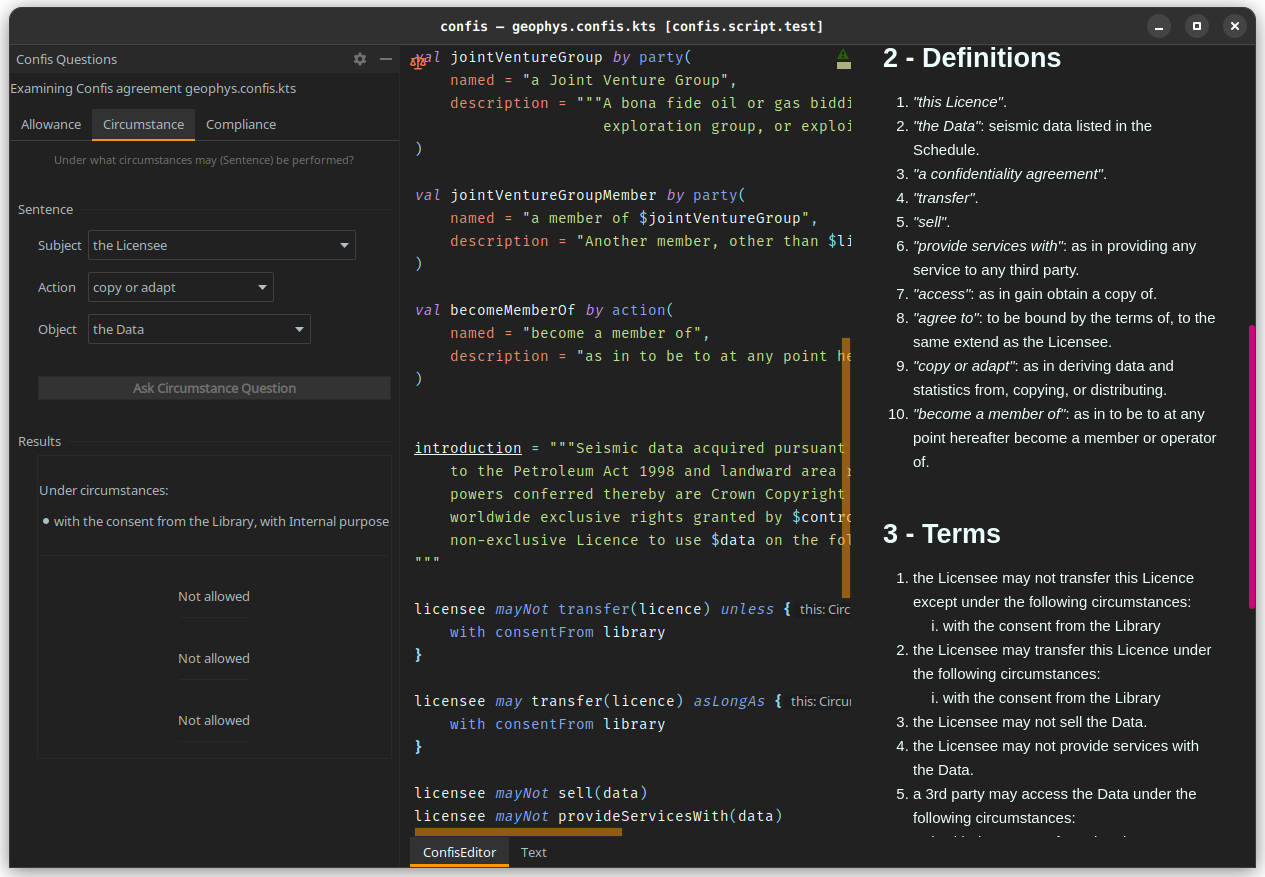
\includegraphics[width=\columnwidth]{figures/confis.full-geophys}
    \caption
    [Screenshot of the Confis Editor and Query UI]
    {Screenshot of the Confis Editor and Query UI, depicting a Confis version of a license for seismic data~\cite{seismicDataLicence}
    \par\footnotesize

    From left to right: the \textbf{Query UI} that allows querying the agreement; the \textbf{Confis code} specifying the agreement; a \textbf{live preview} of the agreement in generated English text.
    }
    \label{fig:geophys-full-editor}
\end{figure}

\autoref{fig:geophys-full-editor} depicts the Confis Editor along with the Query UI


\tikzset{font={\fontsize{9pt}{10}\selectfont}}
\begin{figure}[h]
    \usetikzlibrary{shapes.misc, arrows.meta}
    \colorlet{pastelBlue}{blue!40!white}

    \begin{tikzpicture}
        [
        node distance=2cm and 1.8cm,
        >={Stealth[inset=0pt,length=7pt,angle'=30,round]},
        ]
        \node (user) [
            rectangle,
            rounded corners,
            text=white,
            fill=mdtBlue,
        ] {\textbf{Contract Drafter}};

        \node (docs) [
            draw,
            align=left,
            rectangle,
            rounded corners,
            above=of user,
            rectangle,
        ] {
            \textbf{Online Documentation}\\
            \emph{Uses:}\\HTML pages generated\\from Markdown\\
            \emph{See:}\\\nameref{sec:language-documentation}
        };

        \node (editor) [
            draw,
            text width=3cm,
            rectangle,
            rounded corners,
            below=of user,
            rectangle,
        ] {
            \textbf{Confis Editor}\\
            \emph{Uses:}\\IntelliJ IDEA\\
            \emph{See:}\\\nameref{sec:confis-editor}
        };

        \node (lang) [
            draw,
            rectangle,
            rounded corners,
            text width=4cm,
            left=of editor,
        ] {
            \textbf{Confis Language}\\
            \emph{Uses:}\\Kotlin as host language for DSL\\
            \emph{See:}\\\nameref{sec:language-semantics}
        };

        \node (queryUi) [
            draw,
            text width=3cm,
            rectangle,
            rounded corners,
            right=of editor,
        ] {
            \textbf{Query UI}\\
            \emph{Uses:}\\IntelliJ IDEA\\
            \emph{See:}\\\nameref{sec:queryUI}
        };

        \node (compiler) [
            draw,
            text width=3cm,
            rectangle,
            rounded corners,
            below=of editor,
        ] {
            \textbf{Compiler}\\
            \emph{Uses:}\\Kotlin Compiler\\
            \emph{See:}\\\nameref{subsec:dsl-implementation}
        };

        \node (queryEngine) [
            draw,
            text width=3cm,
            rectangle,
            rounded corners,
            right=of compiler,
        ] {
            \textbf{Query Engine}\\
            \emph{Uses:}\\EasyRules\\
            \emph{See:}\\\nameref{sec:rule-generation}
        };

        \draw[->]
        (user.west)
        to [out=180,in=90]
        node [yshift=0.7cm, text width=6cm]{Formalises agreement into Confis\\semantics as text}
        (lang);

        \draw[->] (lang.east)
        -- node [above, align=center] {Written\\into}
        (editor);

        \draw[->] (editor.270-15)
        -- node[left] { Compiles text }
        (compiler.90+15);

        \draw[->]
        (compiler.90-15)
        -- node[right, text width=3cm] { Compiler\\feedback\\and IR}
        (editor.270+15);

        \draw[->] (editor.north)
        -- node[align=center, fill=white] { Visual feedback }
        (user);

        \draw[->] (editor.east)
        -- node[above, align=center] { Broadcasts\\IR }
        (queryUi);

        \draw[->] (queryUi.270-15)
        -- node[left, text width=2cm, align=right] { IR and\\compiled\\query }
        (queryEngine.90+11);

        \draw[->]
        (queryEngine.90-11)
        -- node[right, text width=3cm] { Query\\result }
        (queryUi.270+15);

        \draw[->]
        (docs.south)
        -- node[align=center, fill=white] { Provides knowledge\\ \& examples }
        (user);

        \draw[->]
        (queryUi.90-15)
        to [out=90,in=10]
        node [above, yshift=0.2cm, fill=white, align=left]{Query rendered\\as English text}
        (user);

        \draw[->]
        (user)
        to [out=-10,in=90]
        node [below, yshift=0.6cm, xshift=-0.8cm, fill=white, align=center]{Query\\selection}
        (queryUi.90+15);

    \end{tikzpicture}
    \caption{Overview of the different components of Confis}
    \label{fig:confis-overview}
\end{figure}
